\documentclass[conference]{IEEEtran}
\IEEEoverridecommandlockouts
% The preceding line is only needed to identify funding in the first footnote. If that is unneeded, please comment it out.
%Template version as of 6/27/2024

\usepackage{cite}
\usepackage{amsmath,amssymb,amsfonts}
\usepackage{algorithmic}
\usepackage{graphicx}
\usepackage{textcomp}
\usepackage{xcolor}
\usepackage{float}
\usepackage[utf8]{inputenc}
\usepackage[T1]{fontenc}
\usepackage[spanish]{babel}


\addto\captionsspanish{
  \renewcommand{\abstractname}{Abstract}
  \renewcommand{\IEEEkeywordsname}{Keywords}
}
\renewcommand{\abstractname}{Abstract}
\renewcommand{\IEEEkeywordsname}{Keywords}
\def\BibTeX{{\rm B\kern-.05em{\sc i\kern-.025em b}\kern-.08em
    T\kern-.1667em\lower.7ex\hbox{E}\kern-.125emX}}
\begin{document}

\title{Análisis de la Densidad Espectral de Potencia en Señales Aleatorias*\\
{\footnotesize \textsuperscript{*} Repositorio de GitHub:}
\thanks{Identify applicable funding agency here. If none, delete this.}
}

\author{\IEEEauthorblockN{1\textsuperscript{st} Edwin Farid Bolaño Perez }
\IEEEauthorblockA{\textit{Codigo: 2212264} \\
\textit{Universidad Industrial de Santander}\\
Bucaramanga, Colombia \\
edwin2212264@correo.uis.edu.co}
\and
\IEEEauthorblockN{2\textsuperscript{nd} Sergio Andres Cardenas}
\IEEEauthorblockA{\textit{Codigo:2222243} \\
\textit{Universidad Industrial de Santander}\\
Bucaramanga, Colombia \\
sergio2222243@correo.uis.edu.co}
\and
\IEEEauthorblockN{3\textsuperscript{rd} Johan Sebastian Fandino Ruiz }
\IEEEauthorblockA{\textit{Codigo:2204271 } \\
\textit{Universidad Industrial de Santander}\\
Bucaramanga, Colombia \\
johan2204271@correo.uis.edu.co}
}

\maketitle

\begin{abstract}
This laboratory practice focuses on the analysis of Power Spectral Density (PSD) 
for random binary signals using software-defined processing. By implementing functional blocks, 
the relationship between Samples per Symbol ($Sps$), bit rate ($R_b$), and spectral bandwidth was characterized for 
bipolar rectangular pulses. Additionally, the spectral behavior of real-world data, including image and audio files, was compared against theoretical white noise models. Results demonstrate
the correlation between temporal parameters and frequency domain energy distribution, reinforcing fundamental concepts of stochastic processes in digital communications.
\end{abstract}

\begin{IEEEkeywords}
component, formatting, style, styling, insert.
\end{IEEEkeywords}

\section{Introduction}
This document is a model and instructions for \LaTeX.
Please observe the conference page limits. For more information about how to become an IEEE Conference author or how to write your paper, please visit   IEEE Conference Author Center website: https://conferences.ieeeauthorcenter.ieee.org/.

\section{Caracterización de Señal Binaria con Diferentes Valores de SPS}
Para el análisis de señales aleatorias, se implementó una fuente de bits con distribución uniforme transformada a un formato bipolar de amplitud $\pm1$. El estudio se centró en la variación sistemática del factor de sobremuestreo ($Sps$), evaluando los valores de $4$, $8$, $16$ y $1$. En cada configuración, se registró el comportamiento de la señal en el dominio del tiempo y se estimó su Densidad Espectral de Potencia (PSD), permitiendo calcular la tasa de bits ($R_b$) y el ancho de banda ocupado.
\begin{figure}[H]
    \centering
    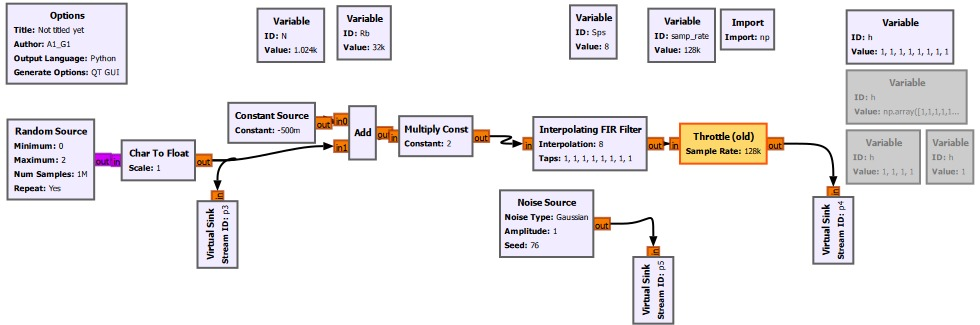
\includegraphics[width=0.5\textwidth]{images/uno.jpeg}
    \caption{Diagrama de bloques de un generador de señales binarias aleatorias bipolar.}
    \label{fig:mi_imagen}
\end{figure}

Antes de proceder a la visualización de los resultados, es fundamental comprender las relaciones y propiedades que rigen los parámetros involucrados en el análisis de señales digitales. El estudio de una señal requiere conocer las características que determinan su comportamiento tanto en el dominio del tiempo como en el de la frecuencia. Parámetros como la tasa de bits ($R_b$), la frecuencia de muestreo ($f_s$) y el ancho de banda ($B$) no solo describen la señal de manera individual, sino que también presentan una relación directa entre sí.

La tasa de bits establece la velocidad de transmisión de la información y puede expresarse como:

\begin{equation}
R_b = \frac{1}{T_b}
\end{equation}

donde $T_b$ corresponde a la duración de cada bit. Por su parte, la frecuencia de muestreo define el número de muestras necesarias para representar la señal, y se obtiene mediante:

\begin{equation}
\text{sample\_rate} = R_b \cdot Sps
\end{equation}

\begin{equation}
f_{s,\text{up}} = Sps \cdot f_{s,\text{sp}}
\end{equation}

Finalmente, el ancho de banda determina el rango de frecuencias necesario para una transmisión adecuada sin pérdidas significativas. En sistemas digitales, este parámetro es clave para evitar errores, ya que las componentes espectrales se distribuyen a lo largo de distintas frecuencias. El ancho de banda se puede calcular como:

\begin{equation}
B = \frac{2 \cdot \text{sample\_rate}}{Sps}
\end{equation}


\begin{figure}[H]
    \centering
    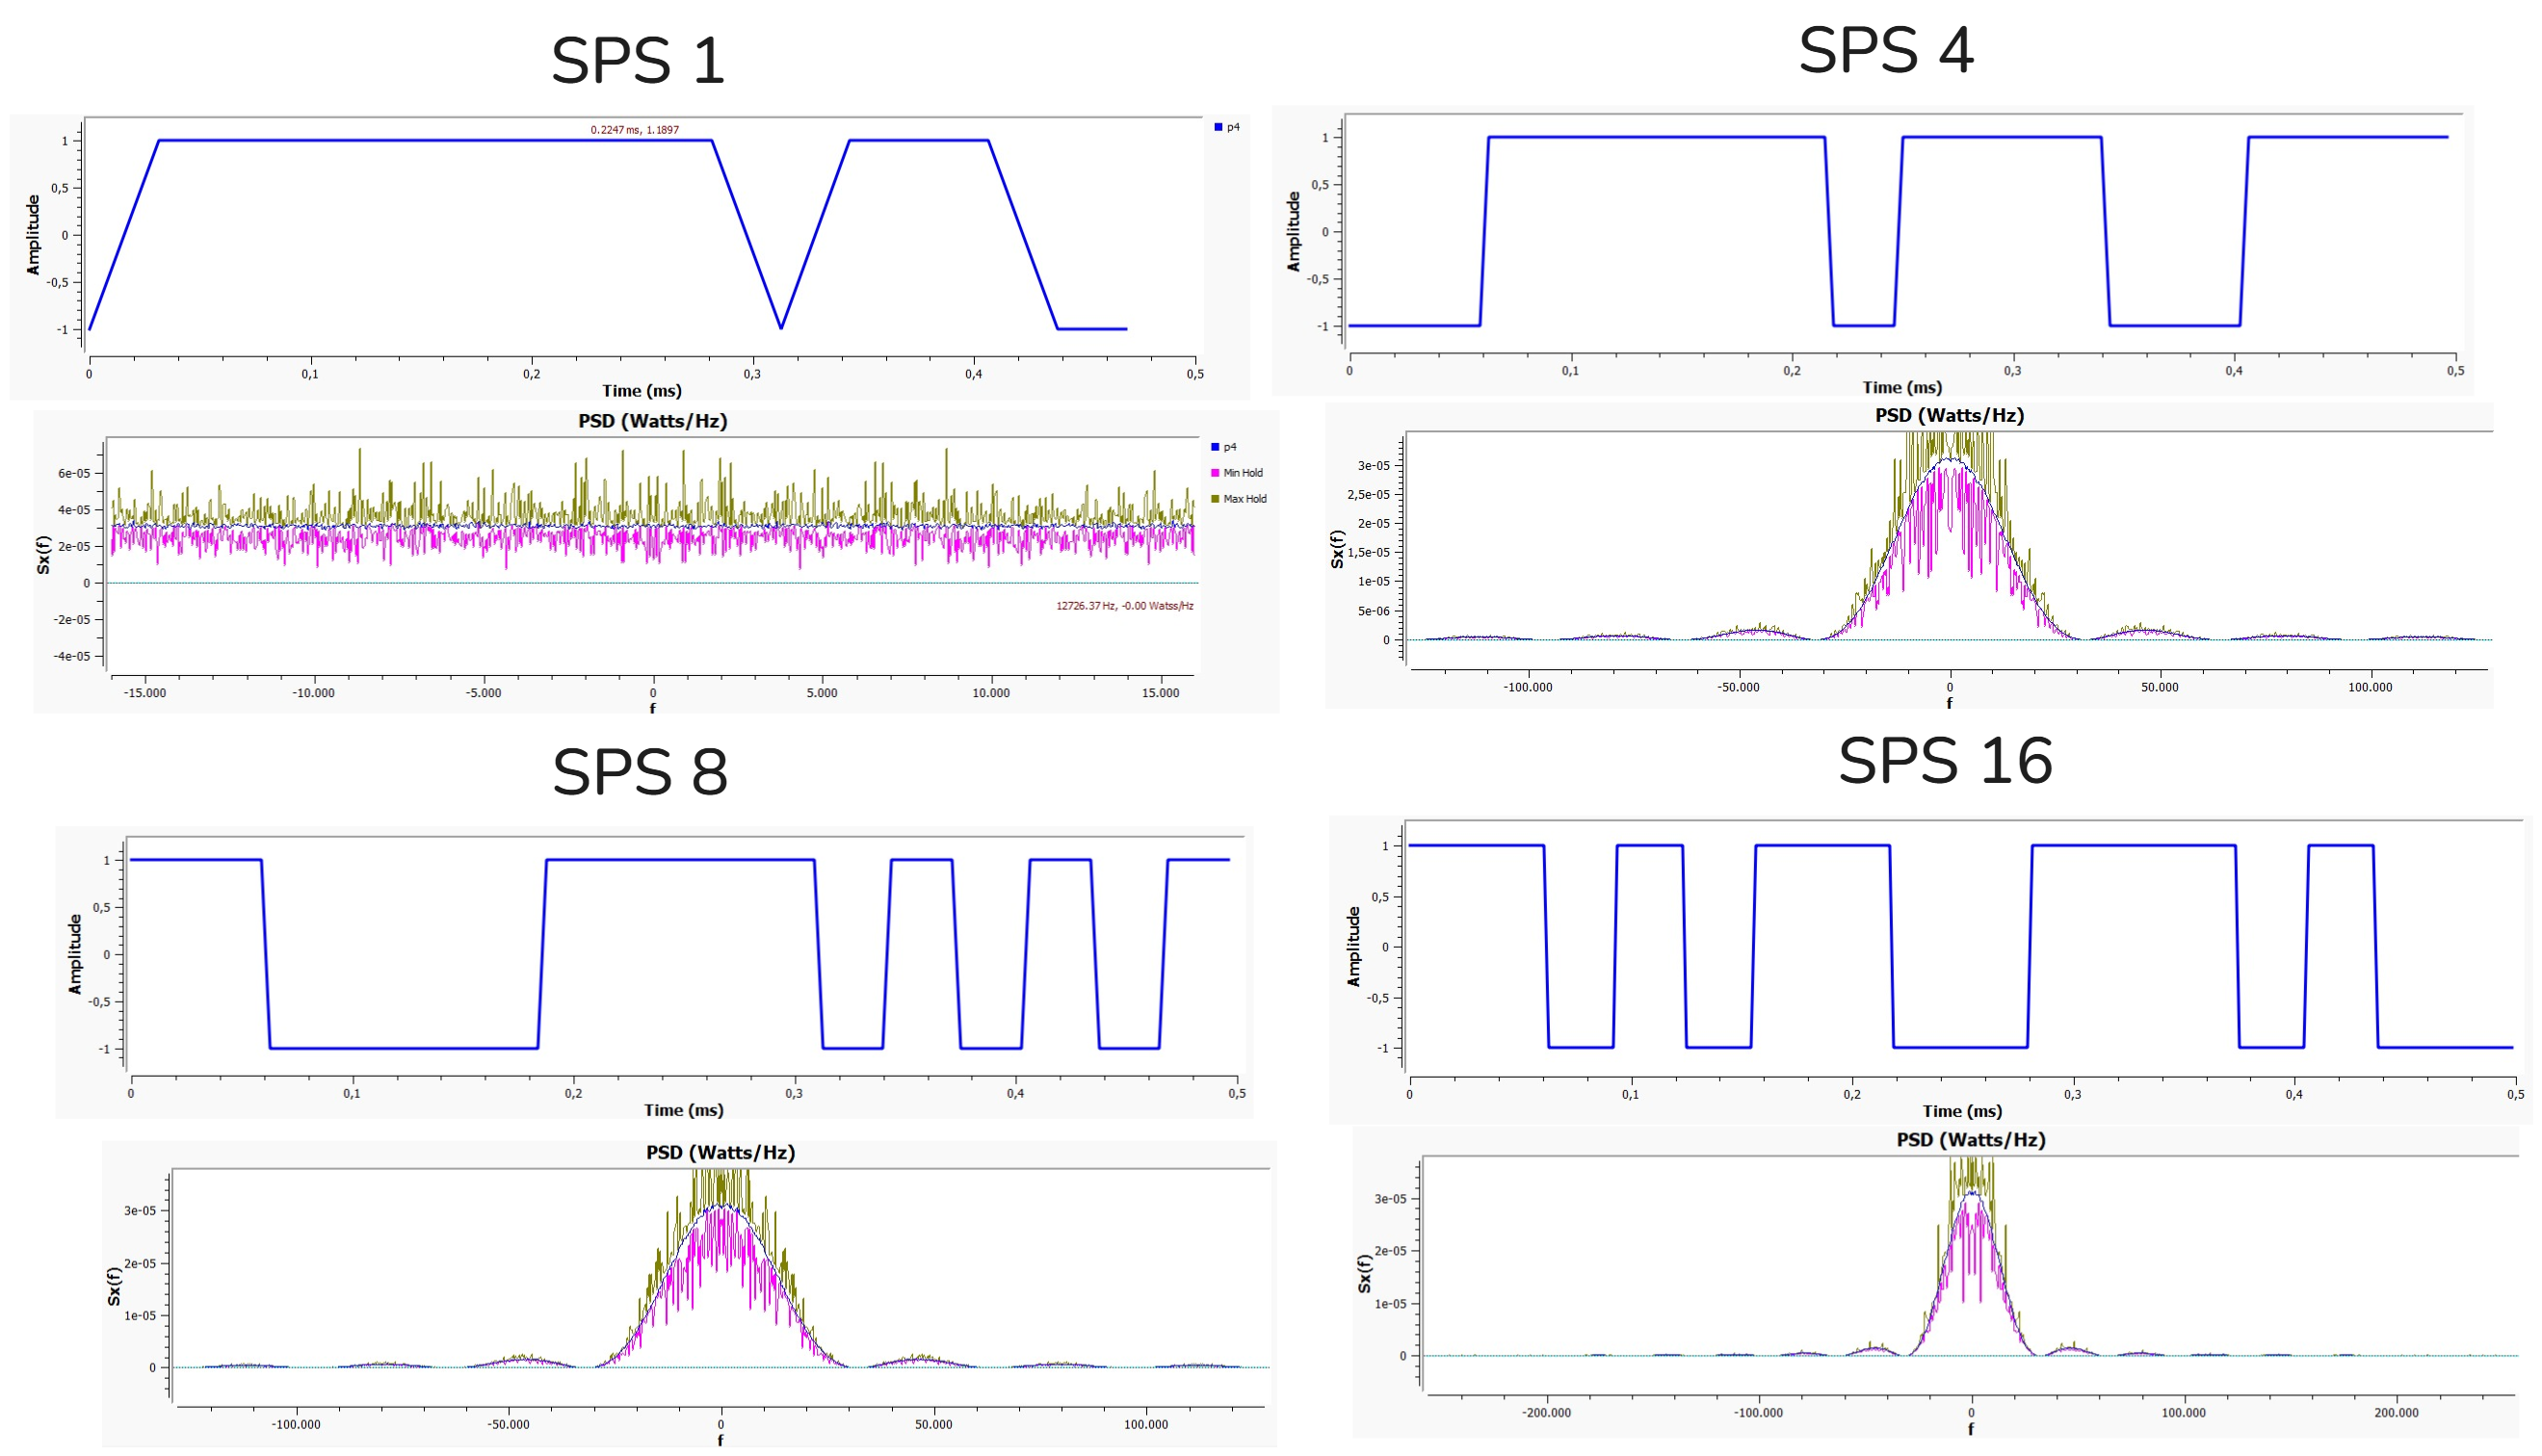
\includegraphics[width=0.5\textwidth]{images/SPS.png}
    \caption{Datos obtenidos}
    \label{fig:mi_imagen}
\end{figure}

\begin{figure}[H]
    \centering
    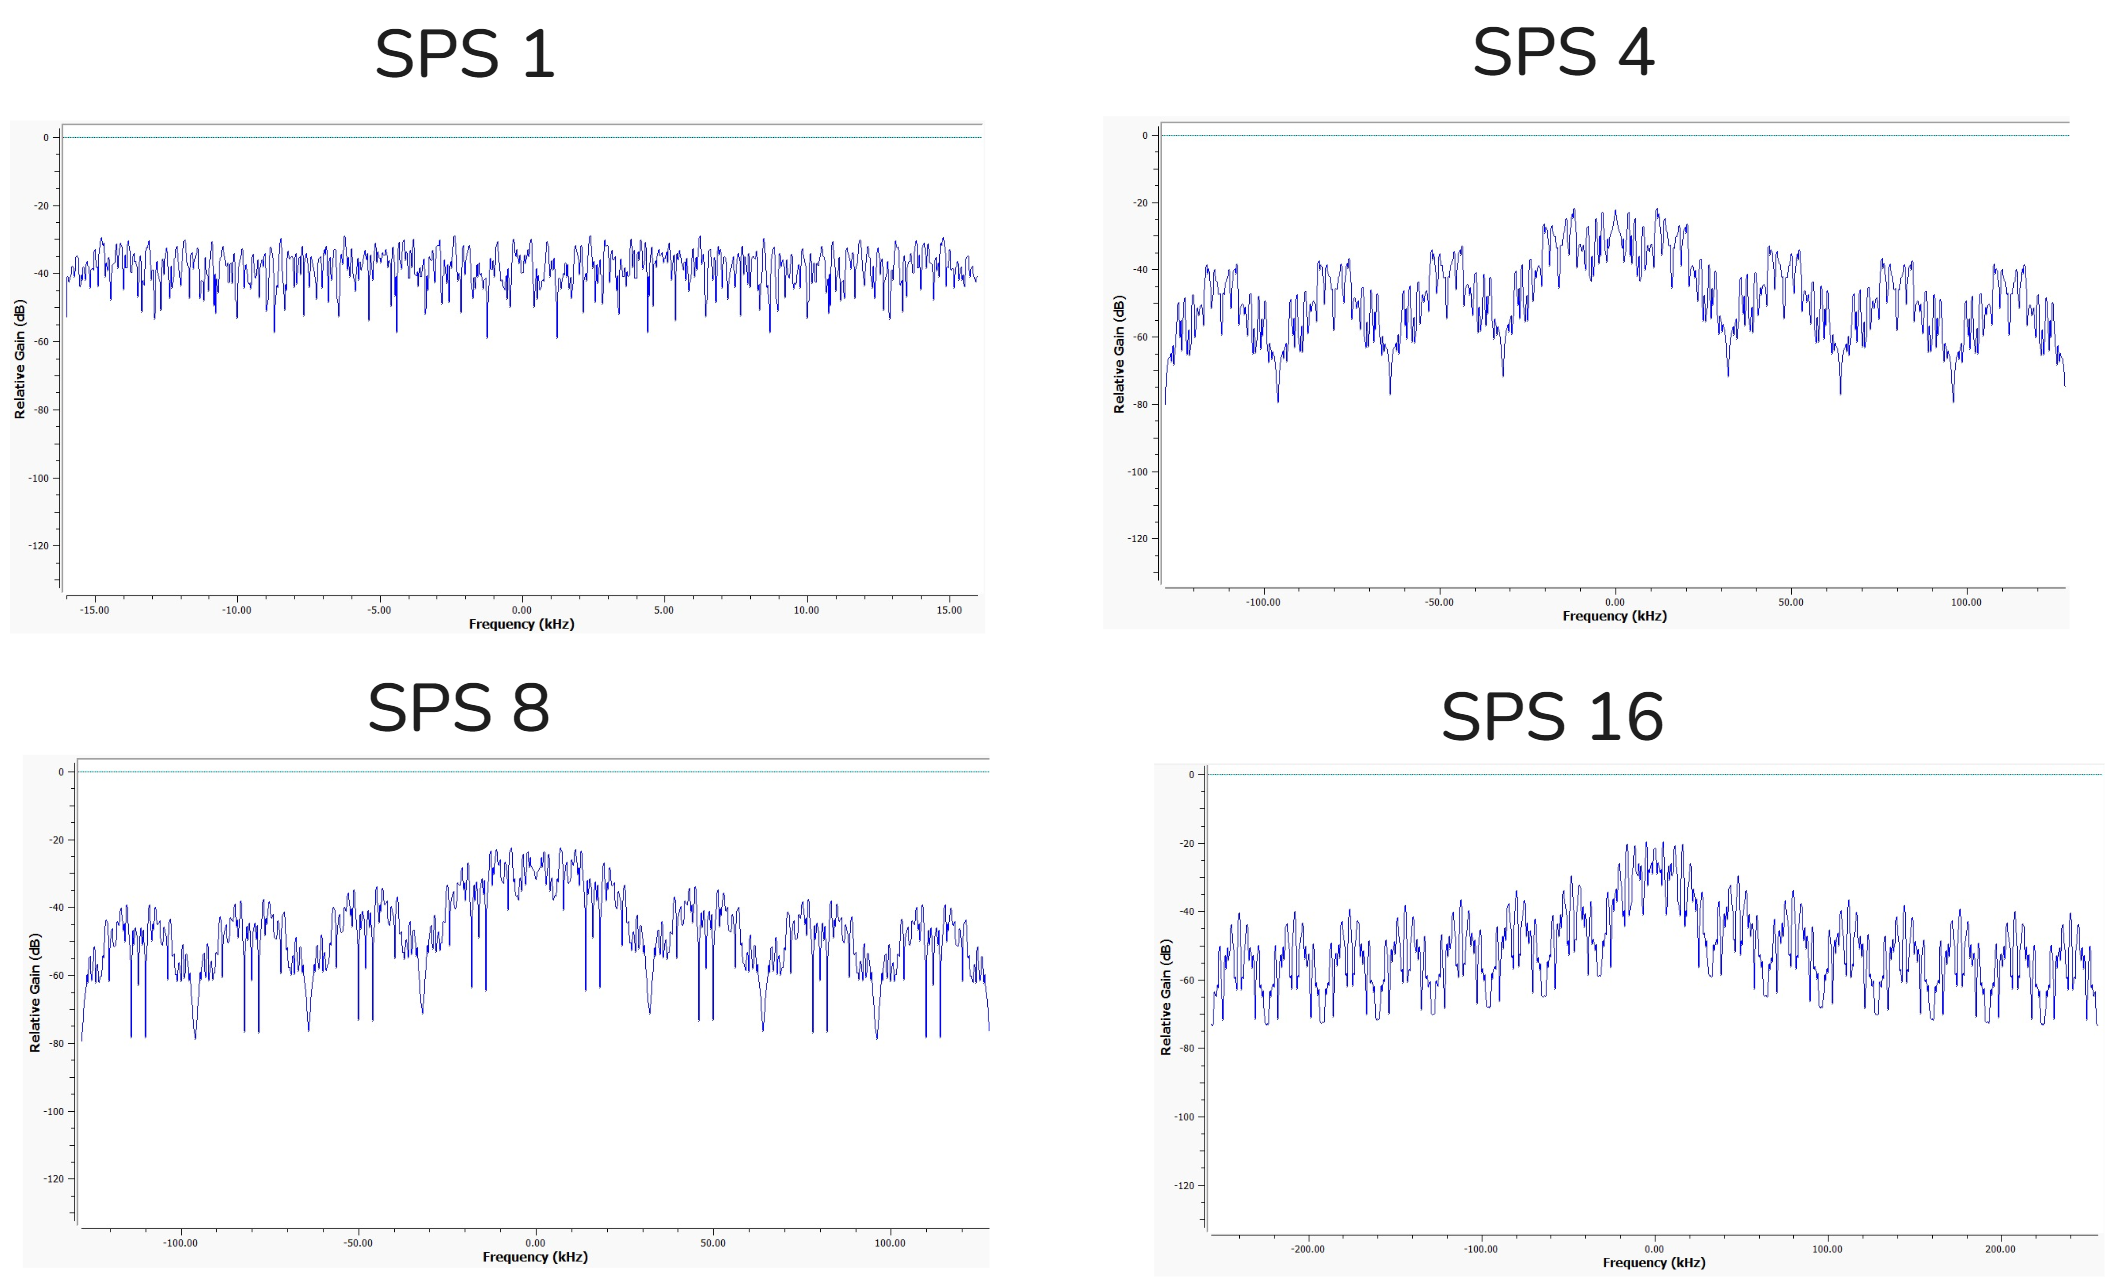
\includegraphics[width=0.4\textwidth]{images/PSD.png}
    \caption{PSD}
    \label{fig:mi_imagen}
\end{figure}
\subsection{Análisis de Resultados: Comportamiento Temporal y Espectral}

A través de la caracterización de la señal binaria aleatoria bipolar ($p4$), se analizó el impacto del sobremuestreo (\textit{Sps}) tanto en el dominio del tiempo como en el de la frecuencia. En el osciloscopio, se observa que al incrementar el valor de \textit{Sps}, los pulsos adquieren una morfología rectangular mucho más nítida y definida; esto representa una mejora significativa en la \textbf{resolución temporal} de la señal digitalizada.

Simultáneamente, en el analizador de espectros, se evidencia que el ancho de banda ($B$) del lóbulo principal de la PSD permanece invariable en 64 kHz, independientemente del valor de sobremuestreo aplicado. Este fenómeno confirma la relación de proporcionalidad directa entre el \textit{Sps} y la frecuencia de muestreo ($f_s$), donde el ajuste dinámico mediante la ecuación:

\begin{equation}
    f_s = R_b \times Sps
\end{equation}

permite compensar el aumento de muestras por símbolo. En conclusión, los resultados consignados en la Tabla \ref{tab:resultados_punto2} validan que la ocupación espectral de la señal depende estrictamente de la tasa de bits ($R_b$).

\begin{table}[h]
\setlength{\tabcolsep}{3pt}
\centering
\small
\caption{Parámetros de la señal binaria según el valor de Sps.}
\label{tab:resultados_punto2}
\begin{tabular}{|c|c|c|c|}
\hline
\textbf{Sps} & \textbf{Rata de bits} & \textbf{Freq. muestreo} & \textbf{Ancho Banda} \\
1            & 32 kbps               & 32 kHz                  & 64 kHz               \\ \hline
4            & 32 kbps               & 128 kHz                 & 64 kHz               \\ \hline
8            & 32 kbps               & 256 kHz                 & 64 kHz               \\ \hline
16           & 32 kbps               & 512 kHz                 & 64 kHz               \\ \hline
\end{tabular}
\end{table}


\section{Análisis del diagrama de bloques para entrada de ruido}
En esta sección se realiza el estudio del comportamiento estocástico del ruido blanco en los dominios del tiempo y la frecuencia. El procedimiento consiste en sustituir la señal binaria por una fuente de ruido aleatorio para evaluar su distribución de energía a través de la Densidad Espectral de Potencia (PSD). Se analiza cómo el factor de sobremuestreo ($Sps$) y el filtrado por interpolación afectan la señal, observando que un incremento en el tamaño del vector del interpolador mejora la resolución temporal y provoca una disminución en el nivel del piso de ruido (\textit{noise floor}).
\begin{figure}[H]
    \centering
    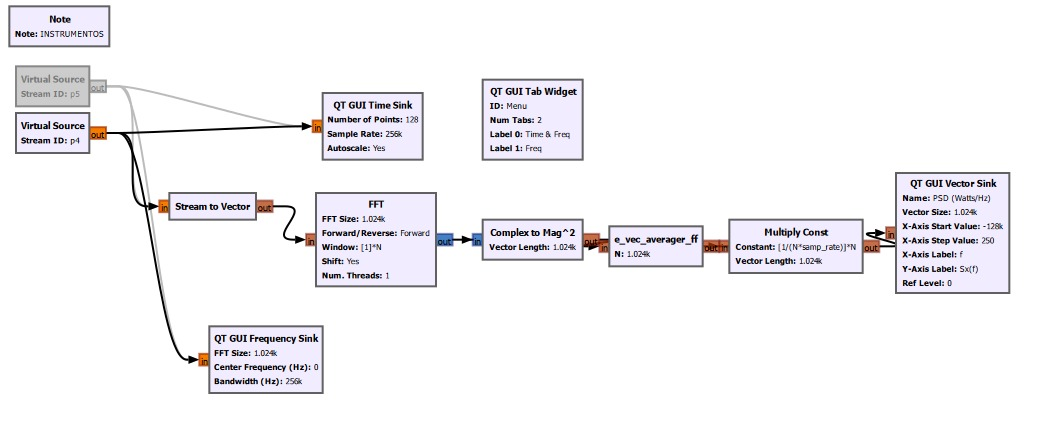
\includegraphics[width=0.5\textwidth]{images/dos.jpeg}
    \caption{Diagrama de bloques que calcula y muestra la densidad de potencia espectral.}
    \label{fig:mi_imagen}
\end{figure}

\begin{figure}[H]
    \centering
    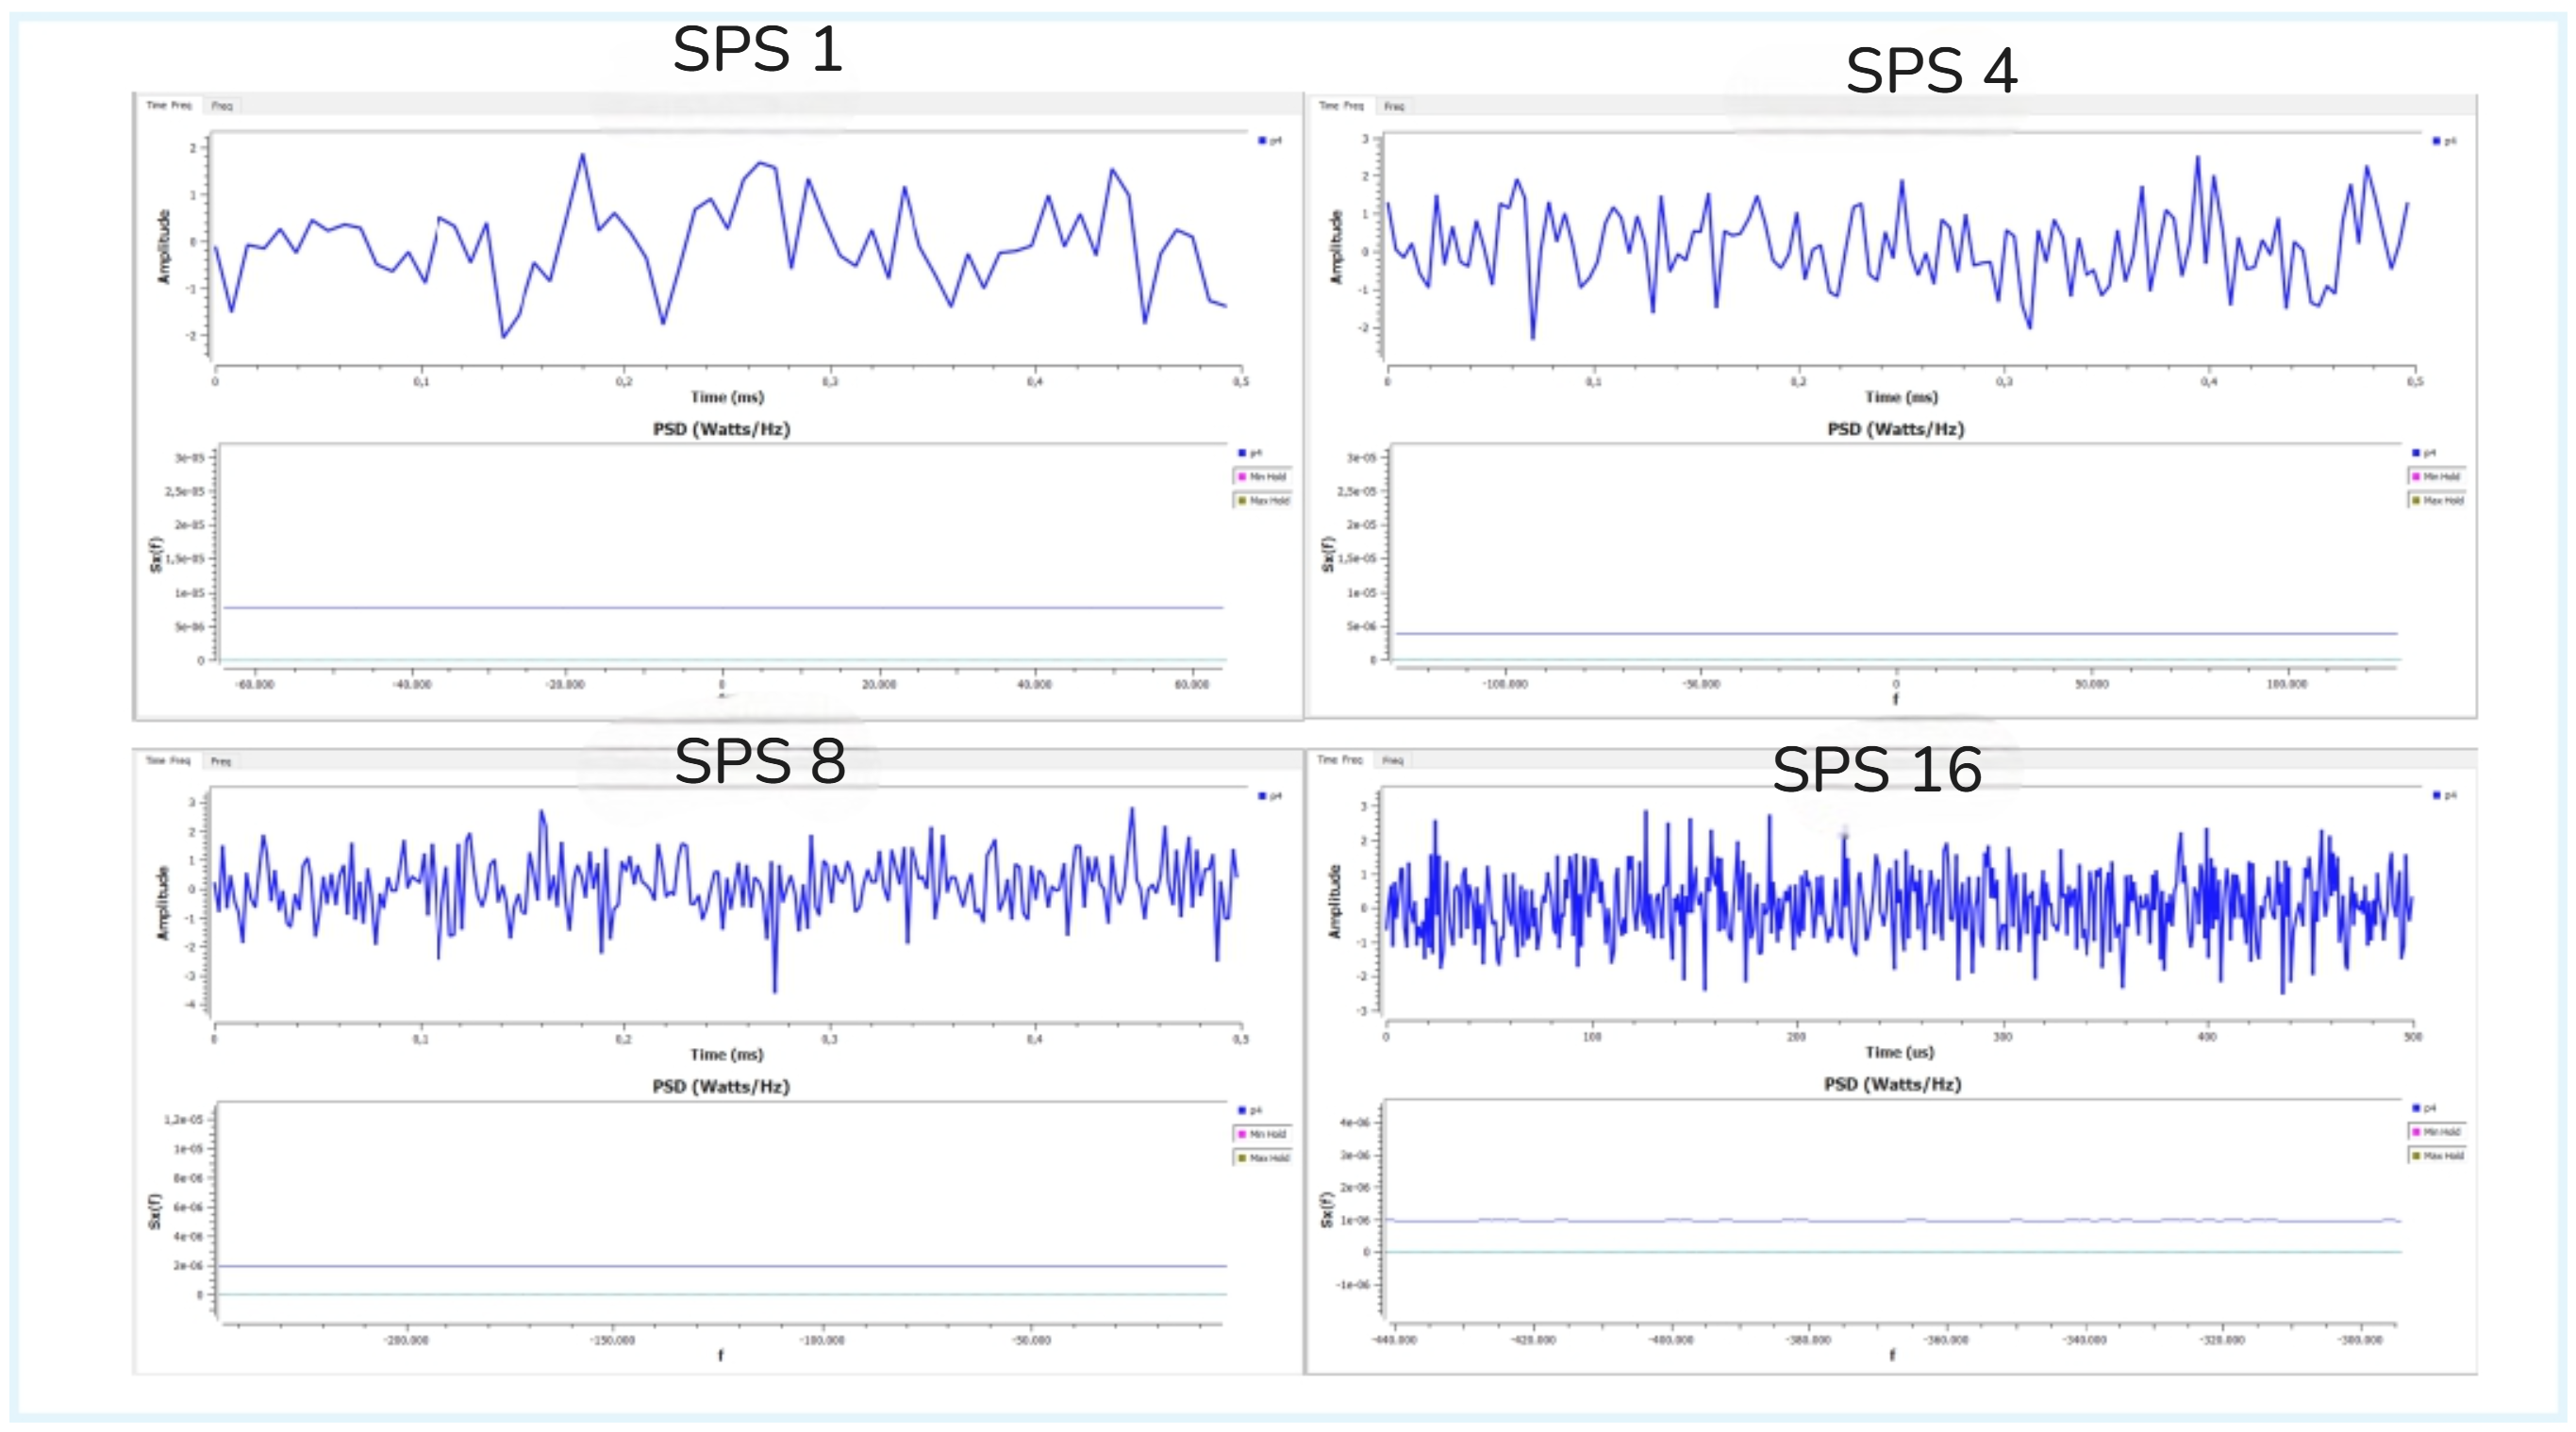
\includegraphics[width=0.5\textwidth]{images/Ruido.png}
    \caption{Analisis de ruido}
    \label{fig:mi_imagen}
\end{figure}


Al incrementar la longitud del vector de coeficientes ($h$) en la operación de convolución, se produce un ensanchamiento de la respuesta en el dominio del tiempo. De acuerdo con las propiedades de la transformada de Fourier, este fenómeno se traduce en una \textbf{mayor selectividad} en el dominio de la frecuencia, lo que equivale a un estrechamiento del ancho de banda de paso del sistema.

Esta mayor selectividad permite filtrar con mayor eficacia las componentes de alta frecuencia, donde se distribuye uniformemente la energía del ruido blanco. En consecuencia, la potencia total del ruido en la señal de salida disminuye, lo cual se refleja experimentalmente como una reducción en el nivel del \textit{noise floor} observado en el análisis de densidad espectral de potencia (PSD).
\section{Análisis de señal proveniente de imagen}

Para este experimento, se reemplazó la fuente de datos aleatoria por una señal proveniente de una imagen, con el objetivo de analizar cómo una fuente real afecta el comportamiento de la señal.

La señal obtenida en el dominio del tiempo mantiene la forma de pulsos rectangulares con niveles bipolares, sin embargo, se evidencian patrones que dependen del contenido de la imagen, lo que indica que no es completamente aleatoria.

\begin{figure}[H]
    \centering
    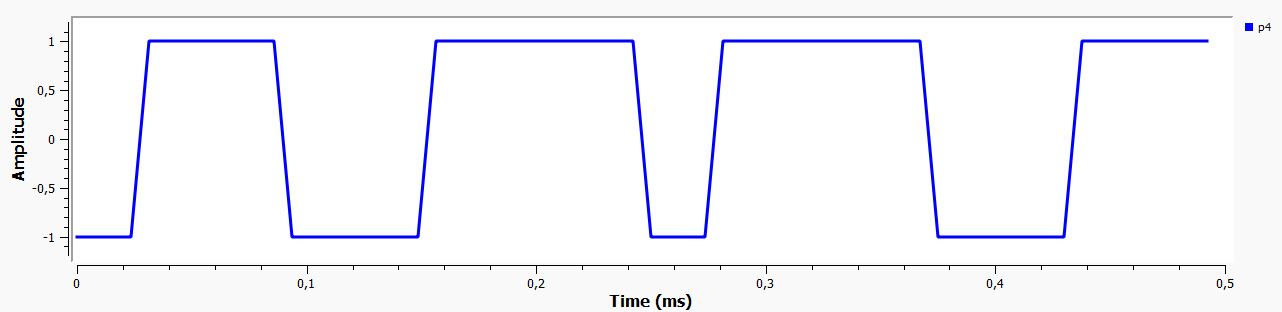
\includegraphics[width=0.5\textwidth]{images/imagen_tiempo.png}
    \caption{Señal en el dominio del tiempo proveniente de una imagen}
\end{figure}

En el dominio de la frecuencia, la densidad espectral de potencia presenta una forma general similar a la de una señal rectangular, pero con irregularidades en su forma.

\begin{figure}[H]
    \centering
    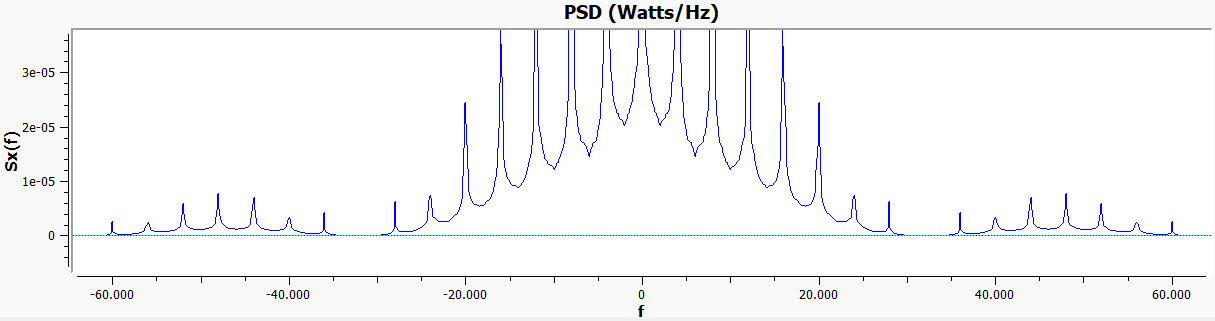
\includegraphics[width=0.5\textwidth]{images/imagen_psd.png}
    \caption{PSD de la señal proveniente de una imagen}
\end{figure}

Estas variaciones indican que la energía no se distribuye de manera uniforme, debido a la correlación presente en los datos de la imagen.

En conclusión, la señal proveniente de una imagen presenta diferencias en su comportamiento espectral respecto a una señal aleatoria, evidenciando la influencia de la fuente de información.

\section{Análisis de señal proveniente de audio}

En este caso, se utilizó una señal proveniente de un archivo de audio, manteniendo el mismo esquema del experimento anterior.

En el dominio del tiempo, la señal conserva la forma de pulsos rectangulares, aunque presenta variaciones más suaves en comparación con una señal aleatoria, lo que refleja la naturaleza de la información de audio.

\begin{figure}[H]
    \centering
    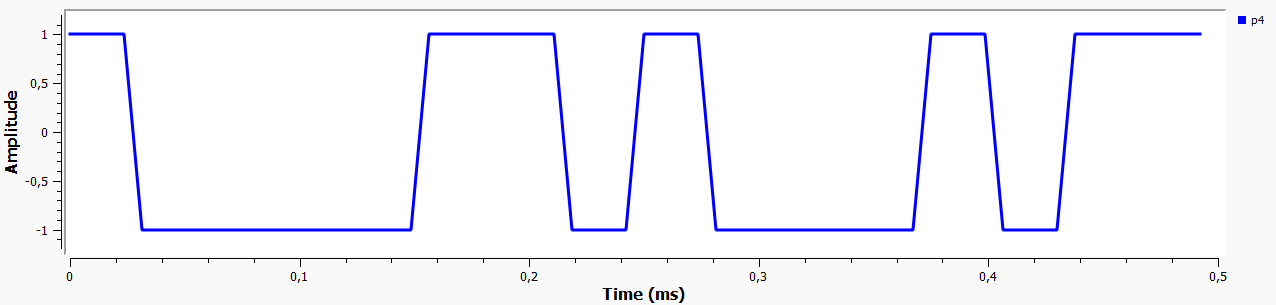
\includegraphics[width=0.5\textwidth]{images/audio_tiempo.png}
    \caption{Señal en el dominio del tiempo proveniente de audio}
\end{figure}

En la densidad espectral de potencia se observa una mayor concentración de energía en bajas frecuencias, lo que indica que la señal presenta variaciones más lentas en el tiempo.

\begin{figure}[H]
    \centering
    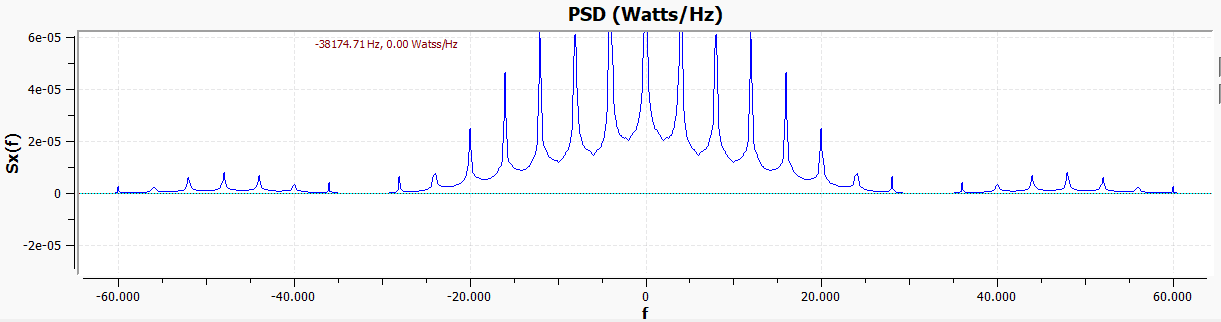
\includegraphics[width=0.5\textwidth]{images/audio_psd.png}
    \caption{PSD de la señal proveniente de audio}
\end{figure}

En conclusión, la señal de audio presenta una distribución espectral diferente, lo cual demuestra que el contenido de la información influye directamente en el comportamiento en frecuencia de la señal.
\section*{References}

Please number citations consecutively within brackets \cite{b1}. The 
sentence punctuation follows the bracket \cite{b2}. Refer simply to the reference 
number, as in \cite{b3}---do not use ``Ref. \cite{b3}'' or ``reference \cite{b3}'' except at 
the beginning of a sentence: ``Reference \cite{b3} was the first $\ldots$''

Number footnotes separately in superscripts. Place the actual footnote at 
the bottom of the column in which it was cited. Do not put footnotes in the 
abstract or reference list. Use letters for table footnotes.

Unless there are six authors or more give all authors' names; do not use 
``et al.''. Papers that have not been published, even if they have been 
submitted for publication, should be cited as ``unpublished'' \cite{b4}. Papers 
that have been accepted for publication should be cited as ``in press'' \cite{b5}. 
Capitalize only the first word in a paper title, except for proper nouns and 
element symbols.

For papers published in translation journals, please give the English 
citation first, followed by the original foreign-language citation \cite{b6}.

\begin{thebibliography}{00}
\bibitem{b1} G. Eason, B. Noble, and I. N. Sneddon, ``On certain integrals of Lipschitz-Hankel type involving products of Bessel functions,'' Phil. Trans. Roy. Soc. London, vol. A247, pp. 529--551, April 1955.
\bibitem{b2} J. Clerk Maxwell, A Treatise on Electricity and Magnetism, 3rd ed., vol. 2. Oxford: Clarendon, 1892, pp.68--73.
\bibitem{b3} I. S. Jacobs and C. P. Bean, ``Fine particles, thin films and exchange anisotropy,'' in Magnetism, vol. III, G. T. Rado and H. Suhl, Eds. New York: Academic, 1963, pp. 271--350.
\bibitem{b4} K. Elissa, ``Title of paper if known,'' unpublished.
\bibitem{b5} R. Nicole, ``Title of paper with only first word capitalized,'' J. Name Stand. Abbrev., in press.
\bibitem{b6} Y. Yorozu, M. Hirano, K. Oka, and Y. Tagawa, ``Electron spectroscopy studies on magneto-optical media and plastic substrate interface,'' IEEE Transl. J. Magn. Japan, vol. 2, pp. 740--741, August 1987 [Digests 9th Annual Conf. Magnetics Japan, p. 301, 1982].
\bibitem{b7} M. Young, The Technical Writer's Handbook. Mill Valley, CA: University Science, 1989.
\bibitem{b8} D. P. Kingma and M. Welling, ``Auto-encoding variational Bayes,'' 2013, arXiv:1312.6114. [Online]. Available: https://arxiv.org/abs/1312.6114
\bibitem{b9} S. Liu, ``Wi-Fi Energy Detection Testbed (12MTC),'' 2023, gitHub repository. [Online]. Available: https://github.com/liustone99/Wi-Fi-Energy-Detection-Testbed-12MTC
\bibitem{b10} ``Treatment episode data set: discharges (TEDS-D): concatenated, 2006 to 2009.'' U.S. Department of Health and Human Services, Substance Abuse and Mental Health Services Administration, Office of Applied Studies, August, 2013, DOI:10.3886/ICPSR30122.v2
\bibitem{b11} K. Eves and J. Valasek, ``Adaptive control for singularly perturbed systems examples,'' Code Ocean, Aug. 2023. [Online]. Available: https://codeocean.com/capsule/4989235/tree
\end{thebibliography}

\vspace{12pt}
\color{red}
IEEE conference templates contain guidance text for composing and formatting conference papers. Please ensure that all template text is removed from your conference paper prior to submission to the conference. Failure to remove the template text from your paper may result in your paper not being published.

\end{document}
